\begin{figure}
\centering
\begin{tabular}{ccc}
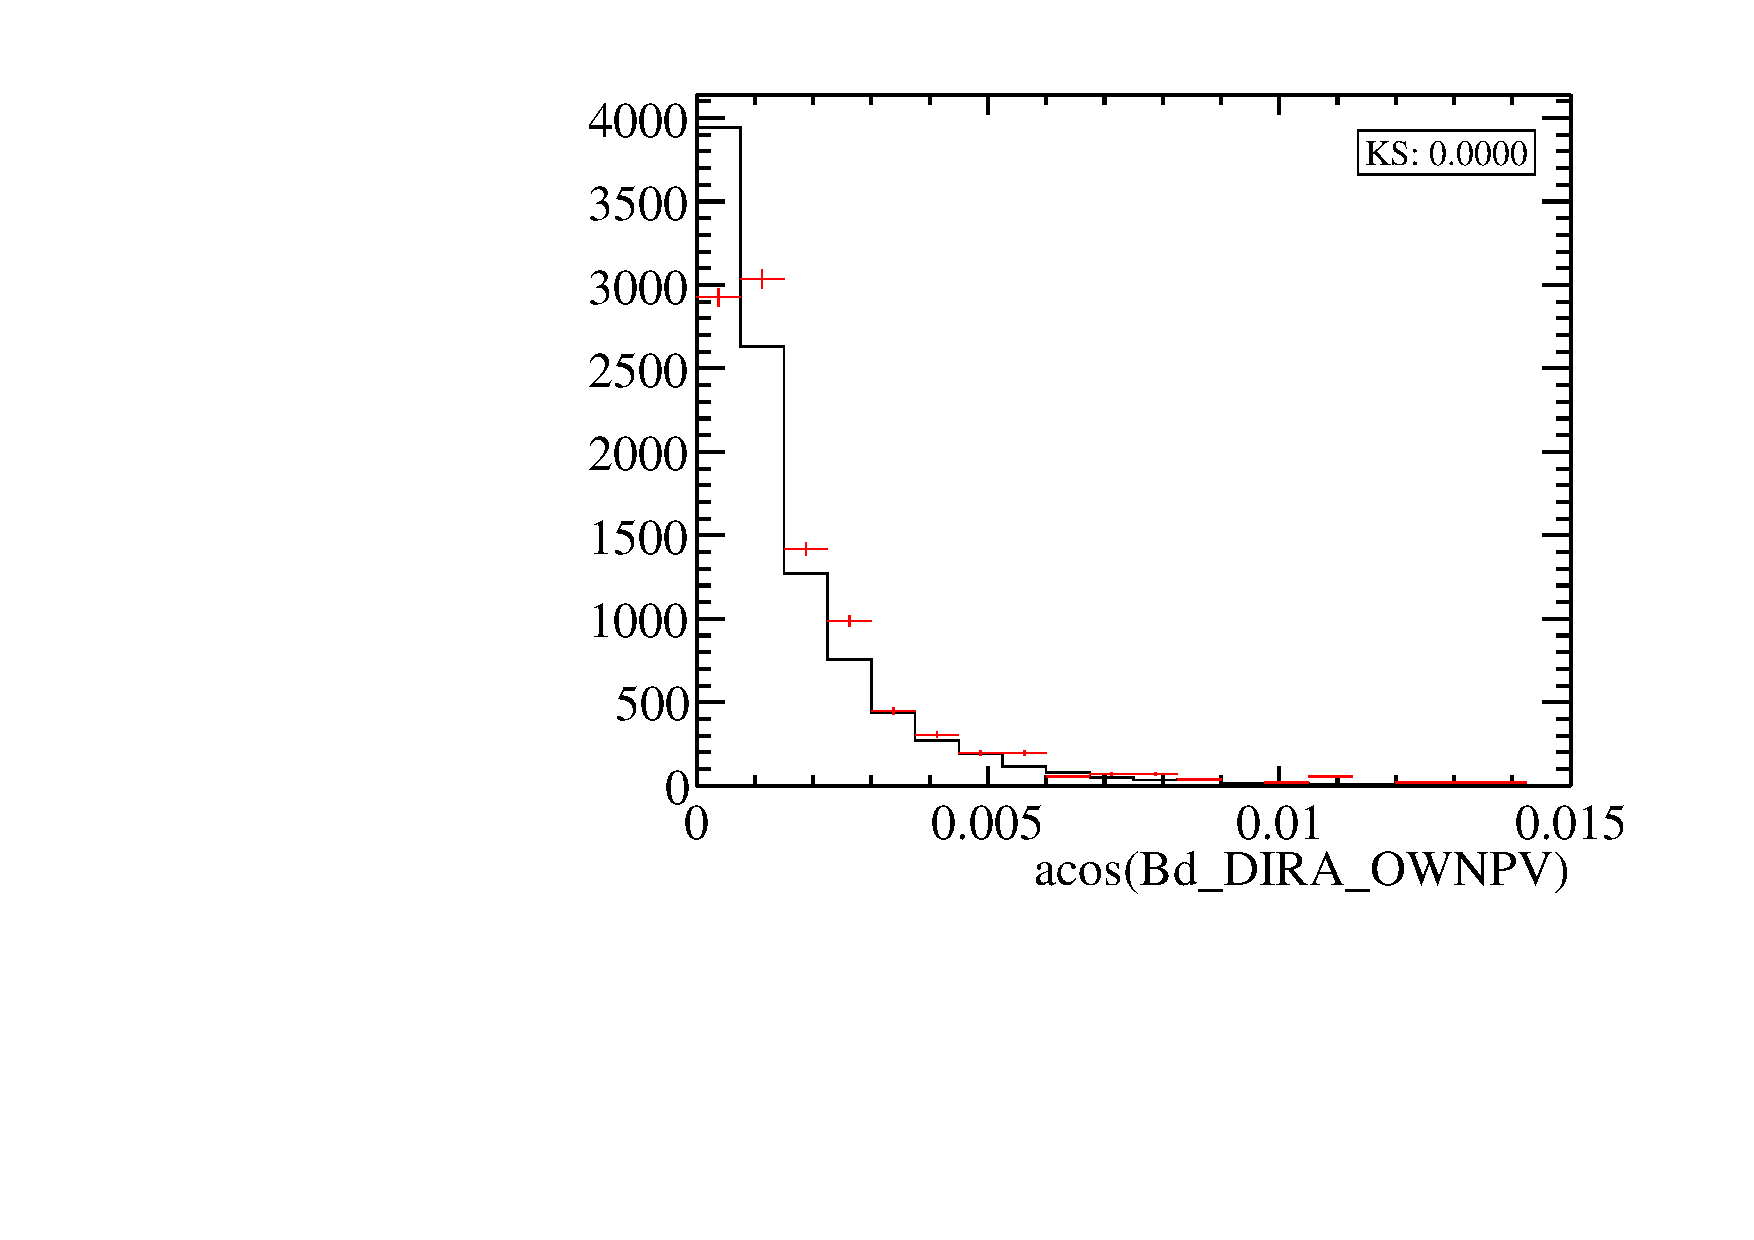
\includegraphics[width=0.3\textwidth]{ANA_resources/Plots/Monte_carlo/data_vs_MC/Kpipipi/acos(Bd_DIRA_OWNPV)_2016.pdf} & 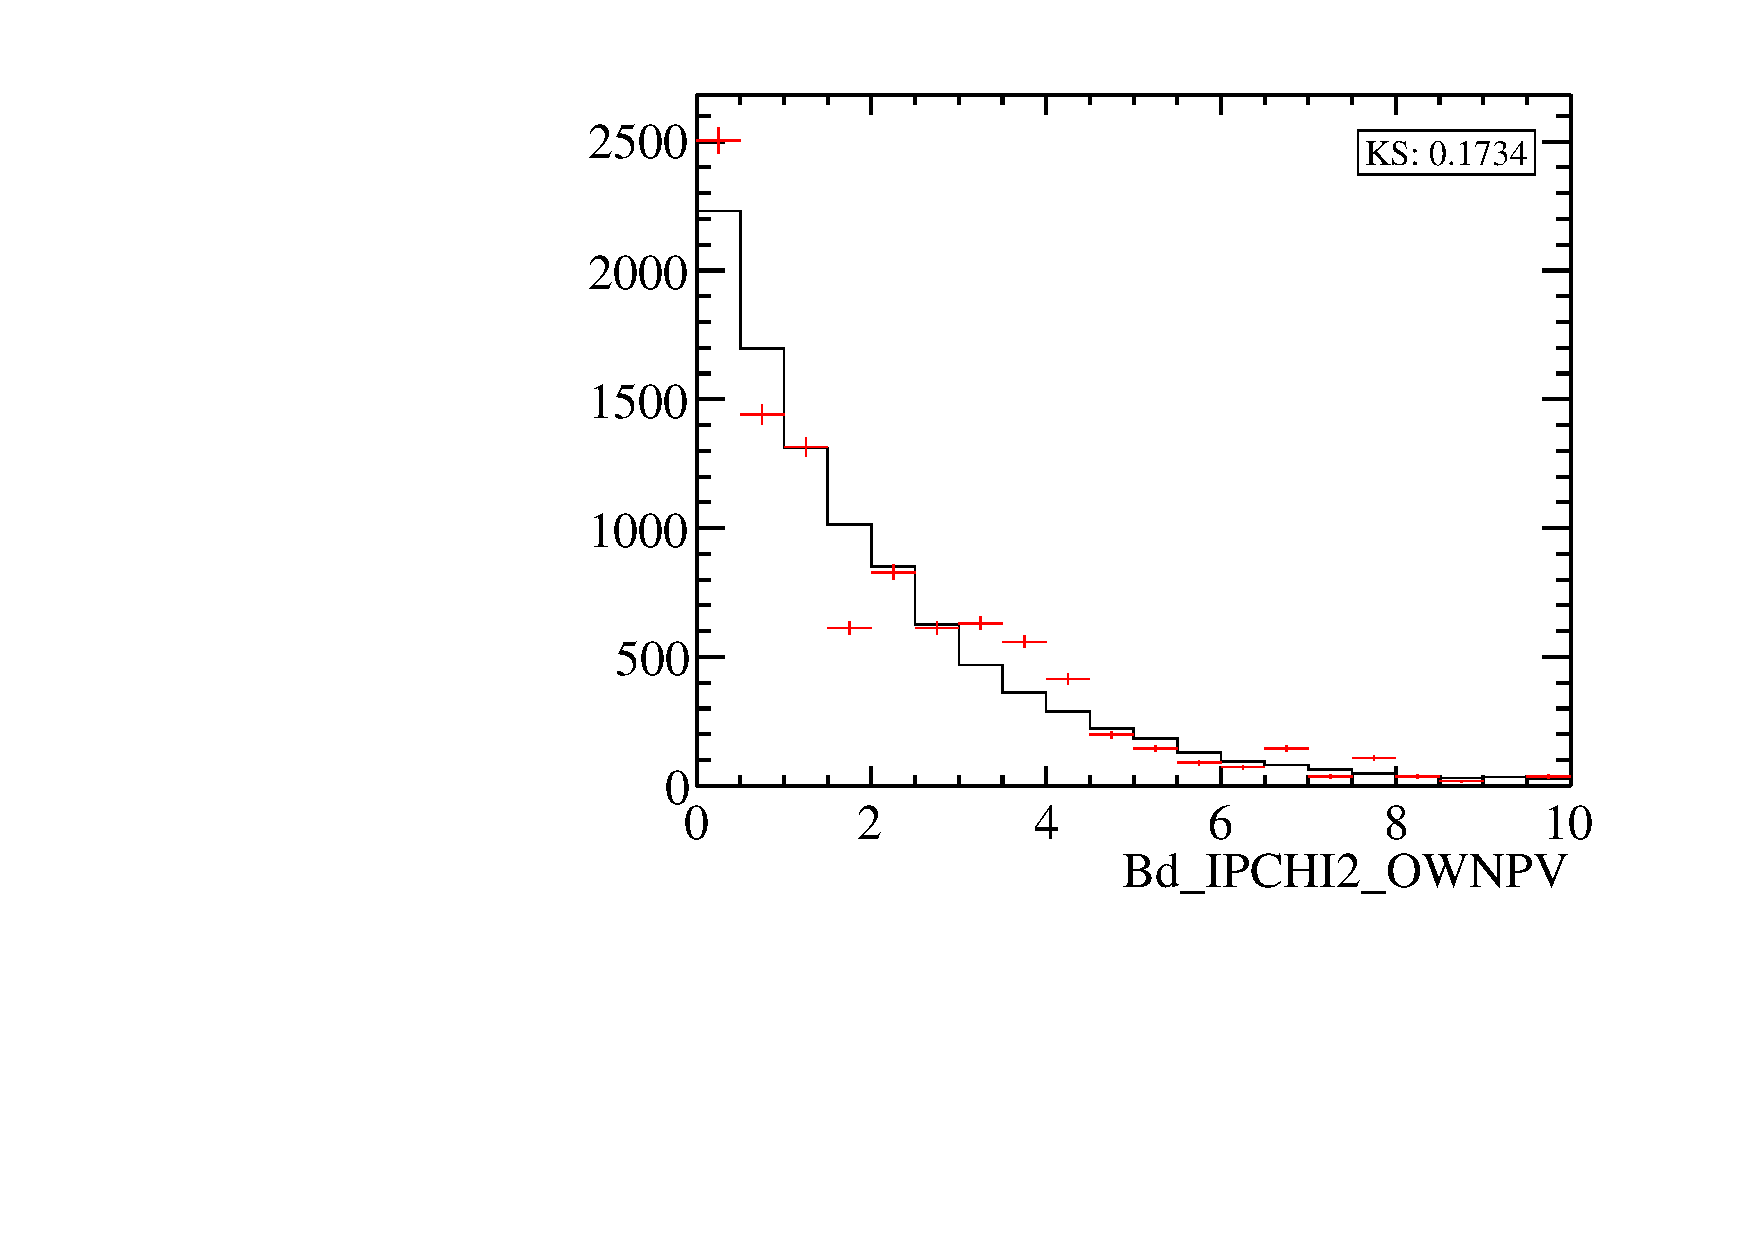
\includegraphics[width=0.3\textwidth]{ANA_resources/Plots/Monte_carlo/data_vs_MC/Kpipipi/Bd_IPCHI2_OWNPV_2016.pdf} & 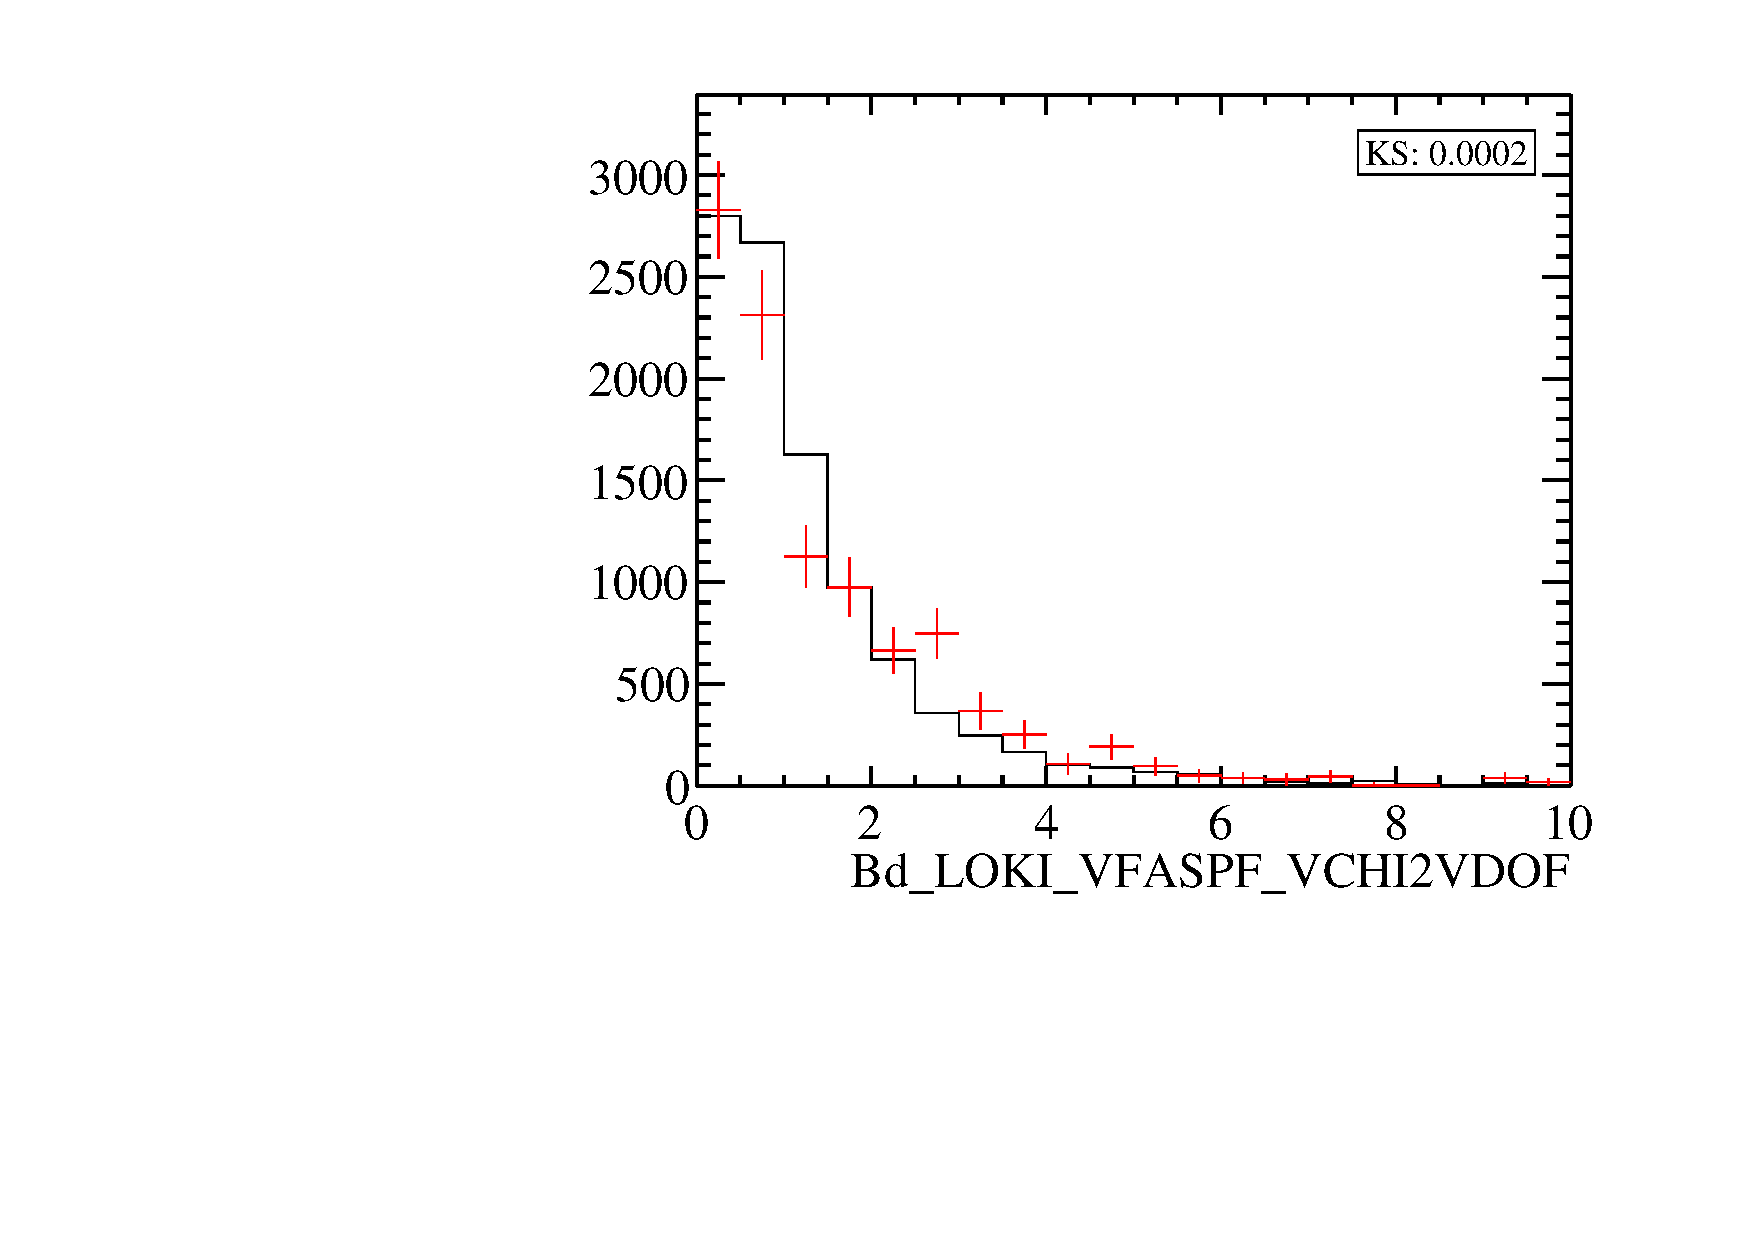
\includegraphics[width=0.3\textwidth]{ANA_resources/Plots/Monte_carlo/data_vs_MC/Kpipipi/Bd_LOKI_VFASPF_VCHI2VDOF_2016.pdf} \\
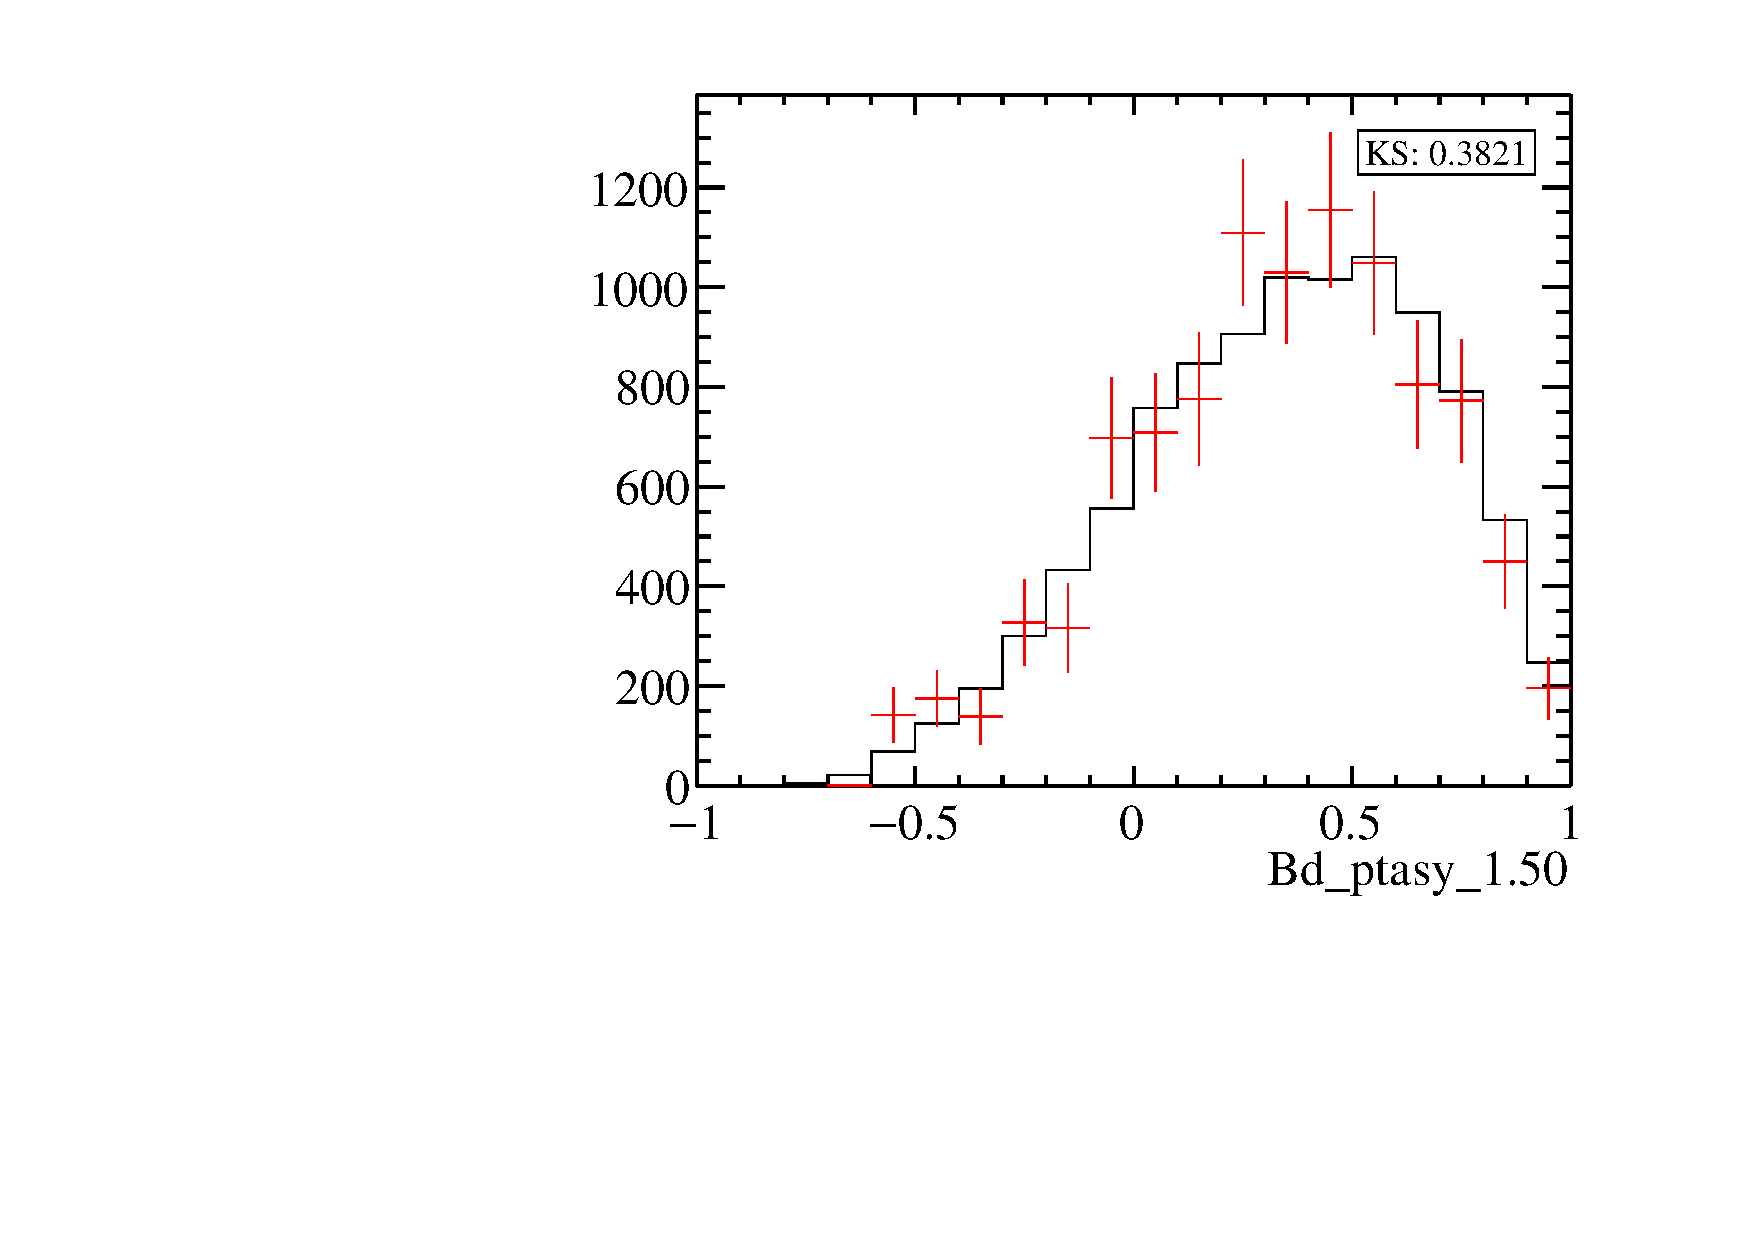
\includegraphics[width=0.3\textwidth]{ANA_resources/Plots/Monte_carlo/data_vs_MC/Kpipipi/Bd_ptasy_1_50_2016.pdf} & 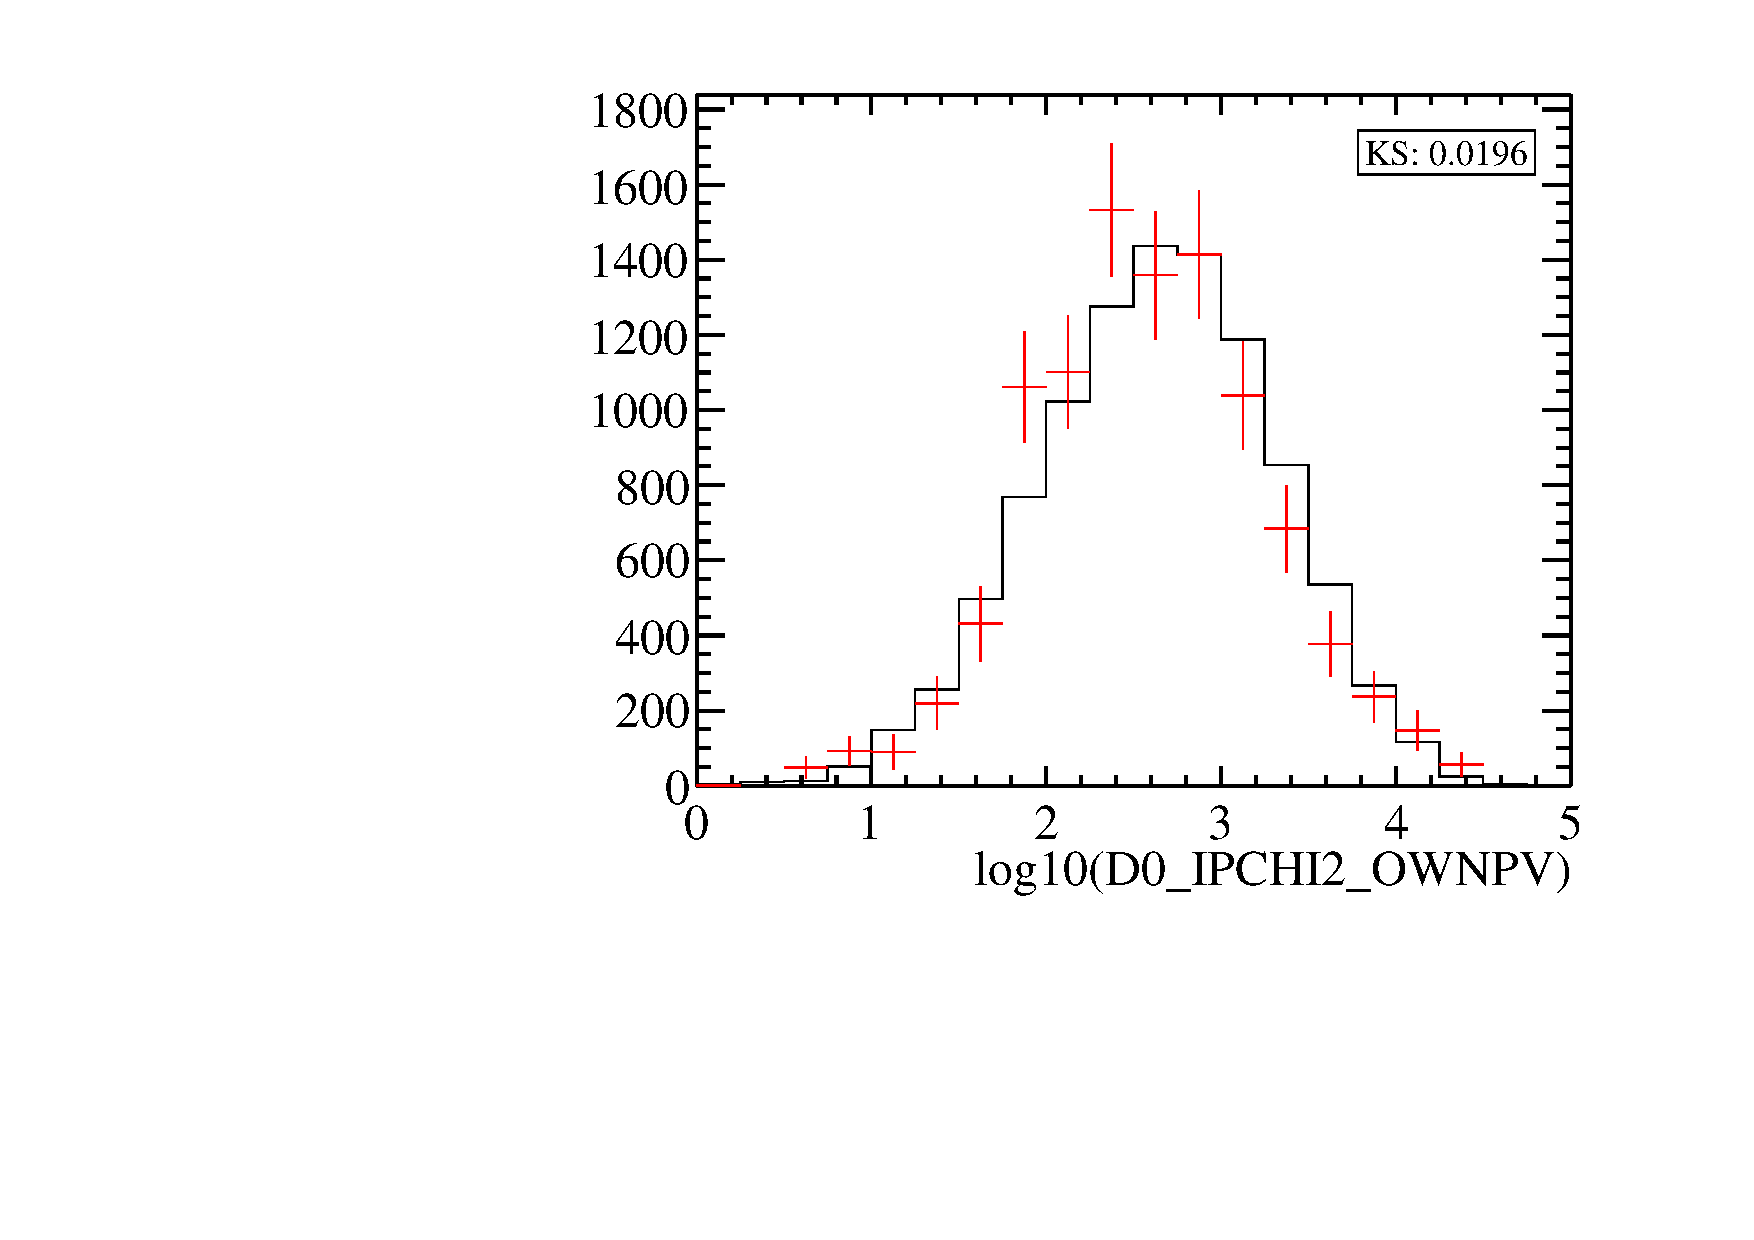
\includegraphics[width=0.3\textwidth]{ANA_resources/Plots/Monte_carlo/data_vs_MC/Kpipipi/log10(D0_IPCHI2_OWNPV)_2016.pdf} & 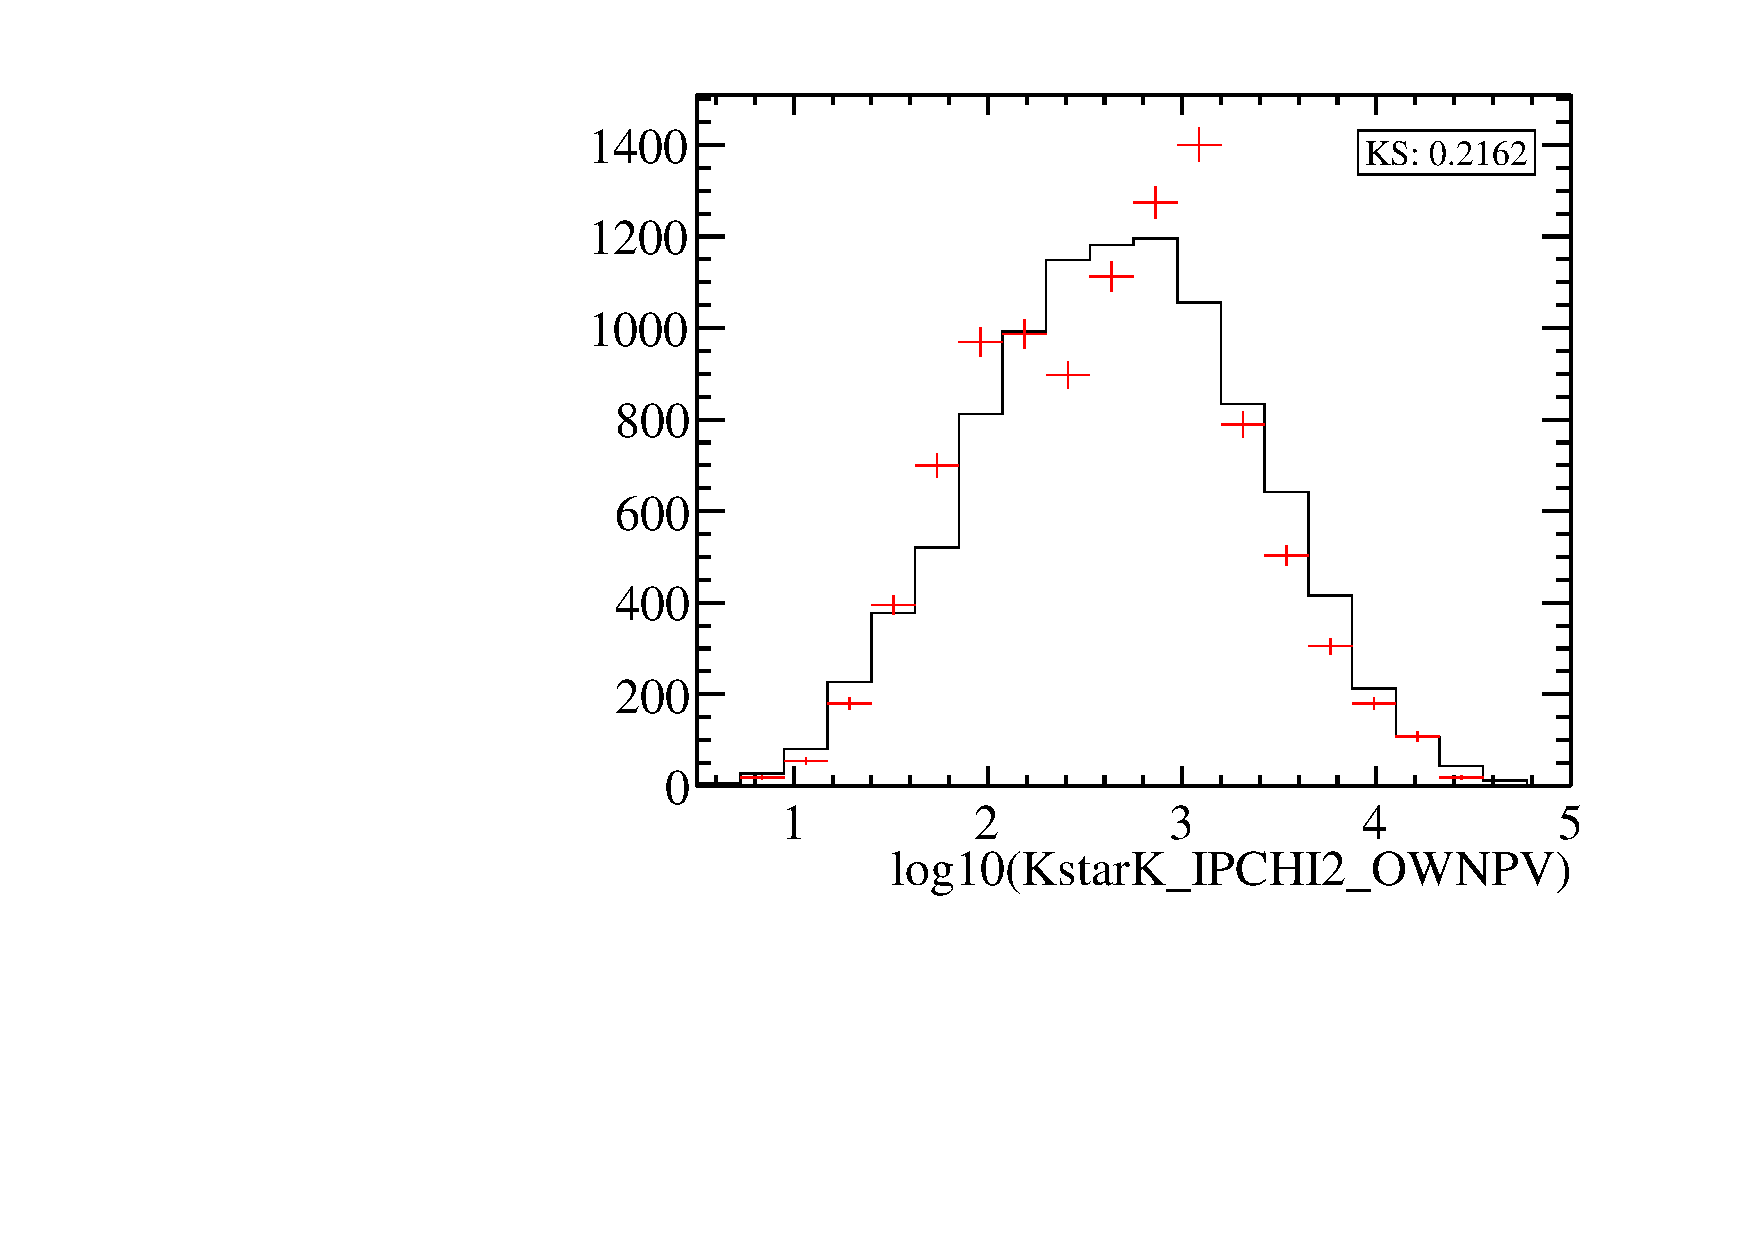
\includegraphics[width=0.3\textwidth]{ANA_resources/Plots/Monte_carlo/data_vs_MC/Kpipipi/log10(KstarK_IPCHI2_OWNPV)_2016.pdf} \\
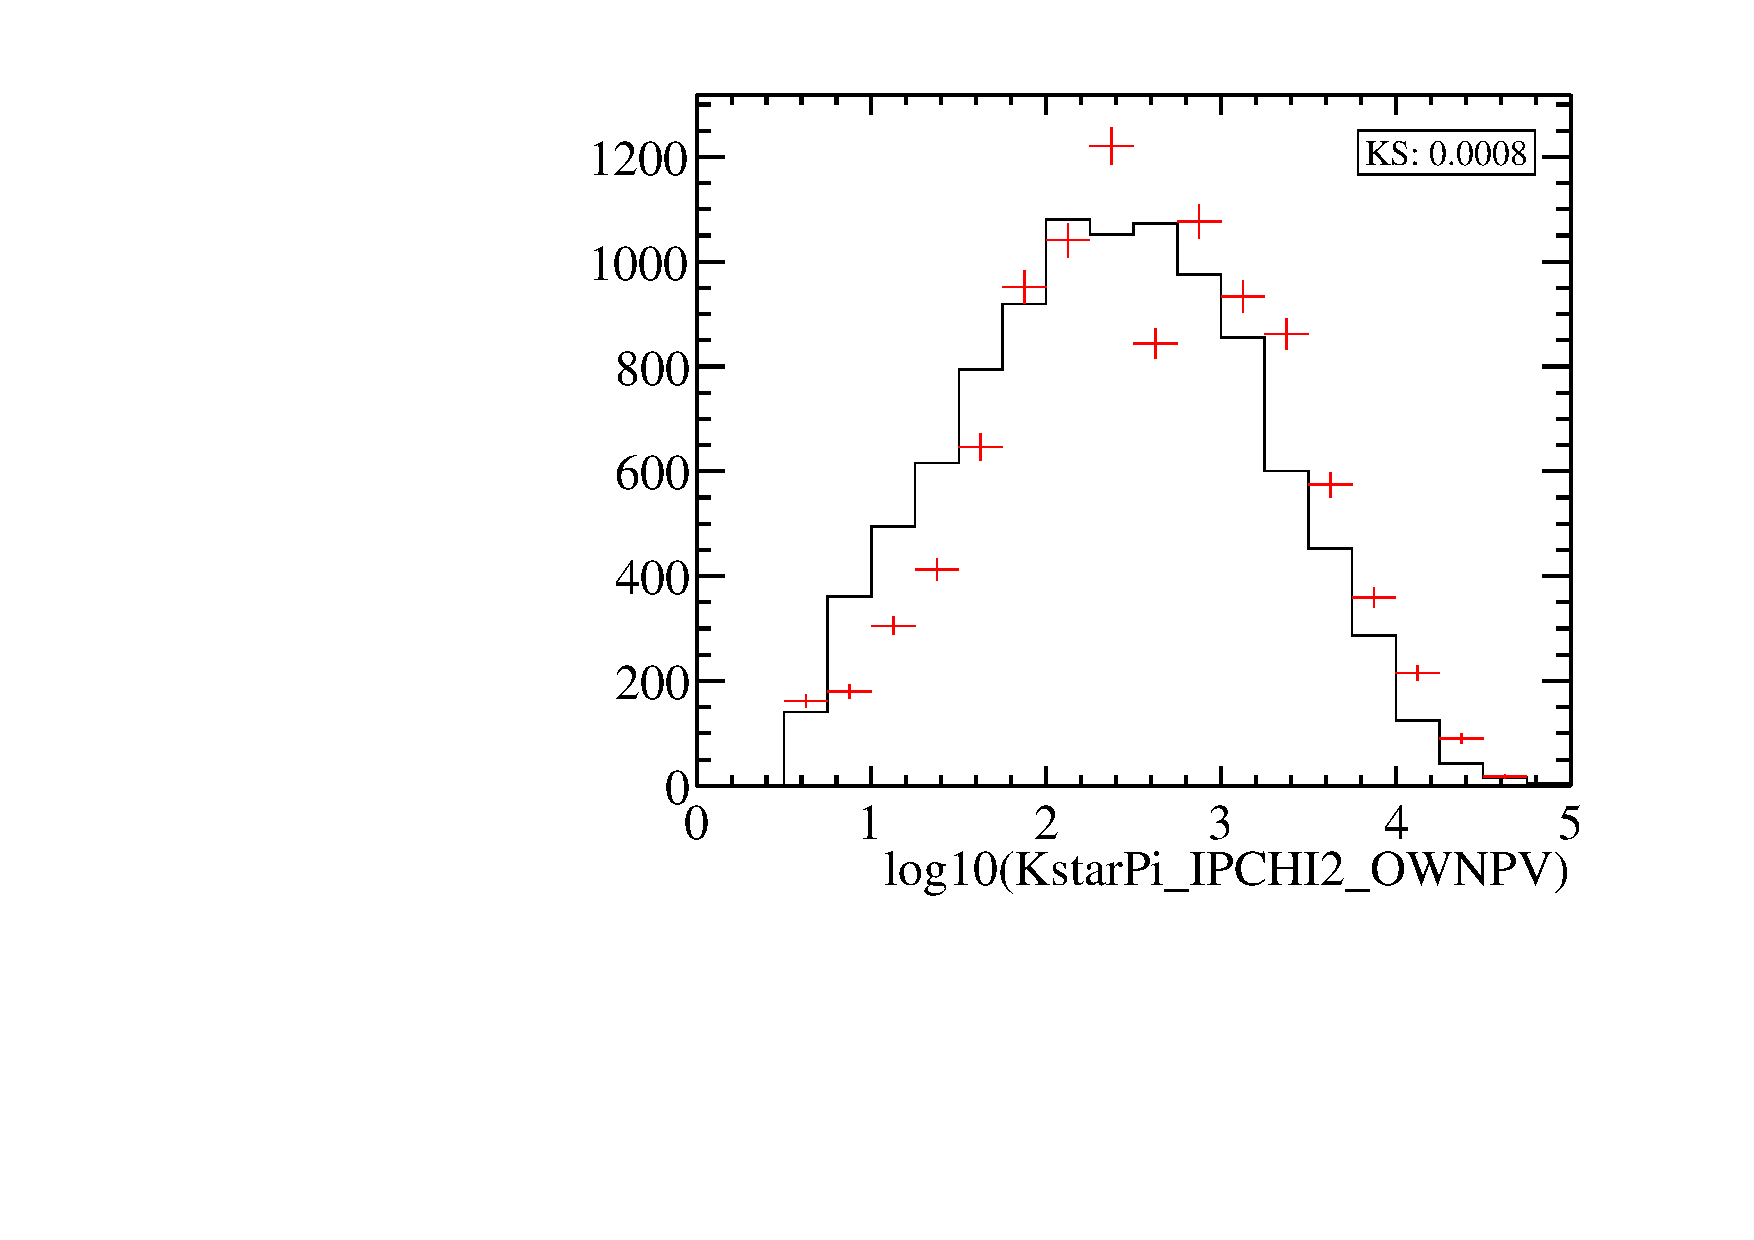
\includegraphics[width=0.3\textwidth]{ANA_resources/Plots/Monte_carlo/data_vs_MC/Kpipipi/log10(KstarPi_IPCHI2_OWNPV)_2016.pdf} & 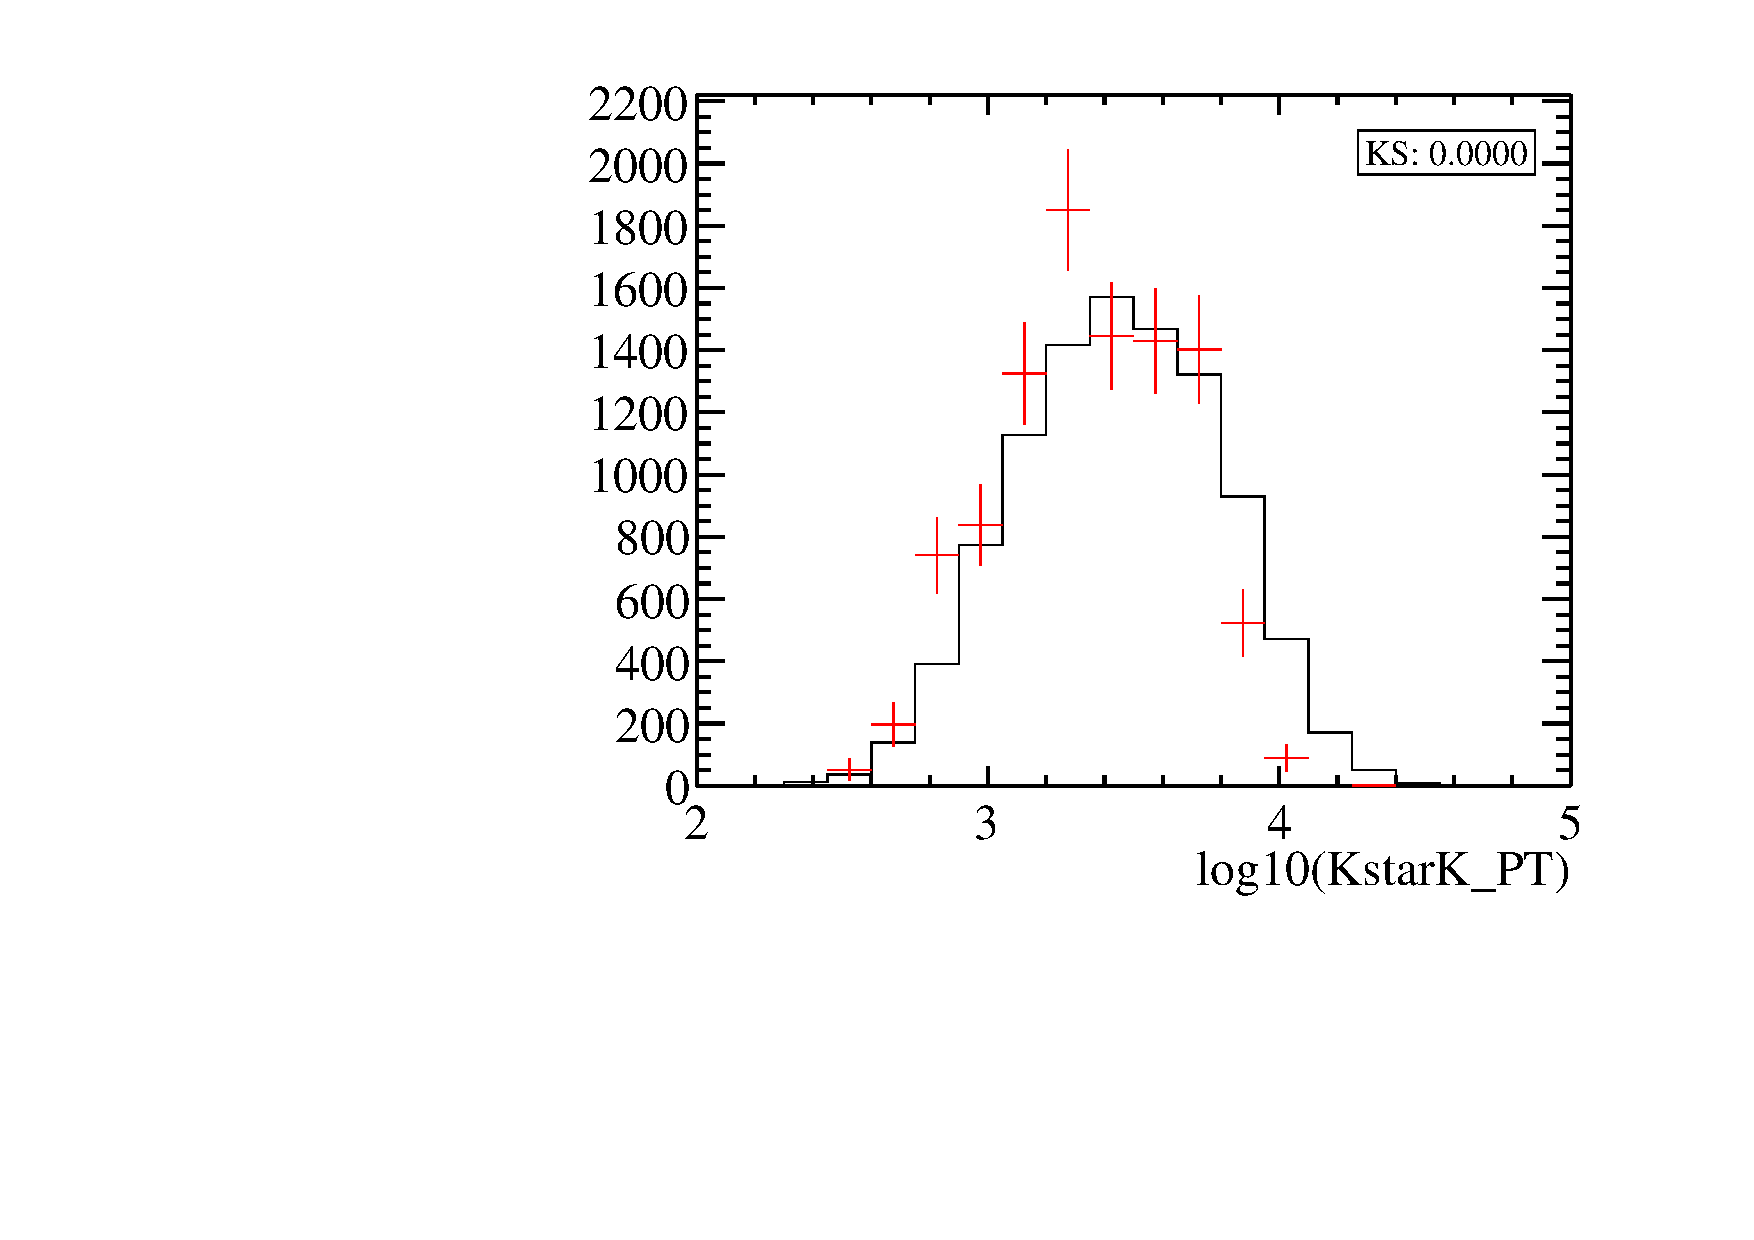
\includegraphics[width=0.3\textwidth]{ANA_resources/Plots/Monte_carlo/data_vs_MC/Kpipipi/log10(KstarK_PT)_2016.pdf} & 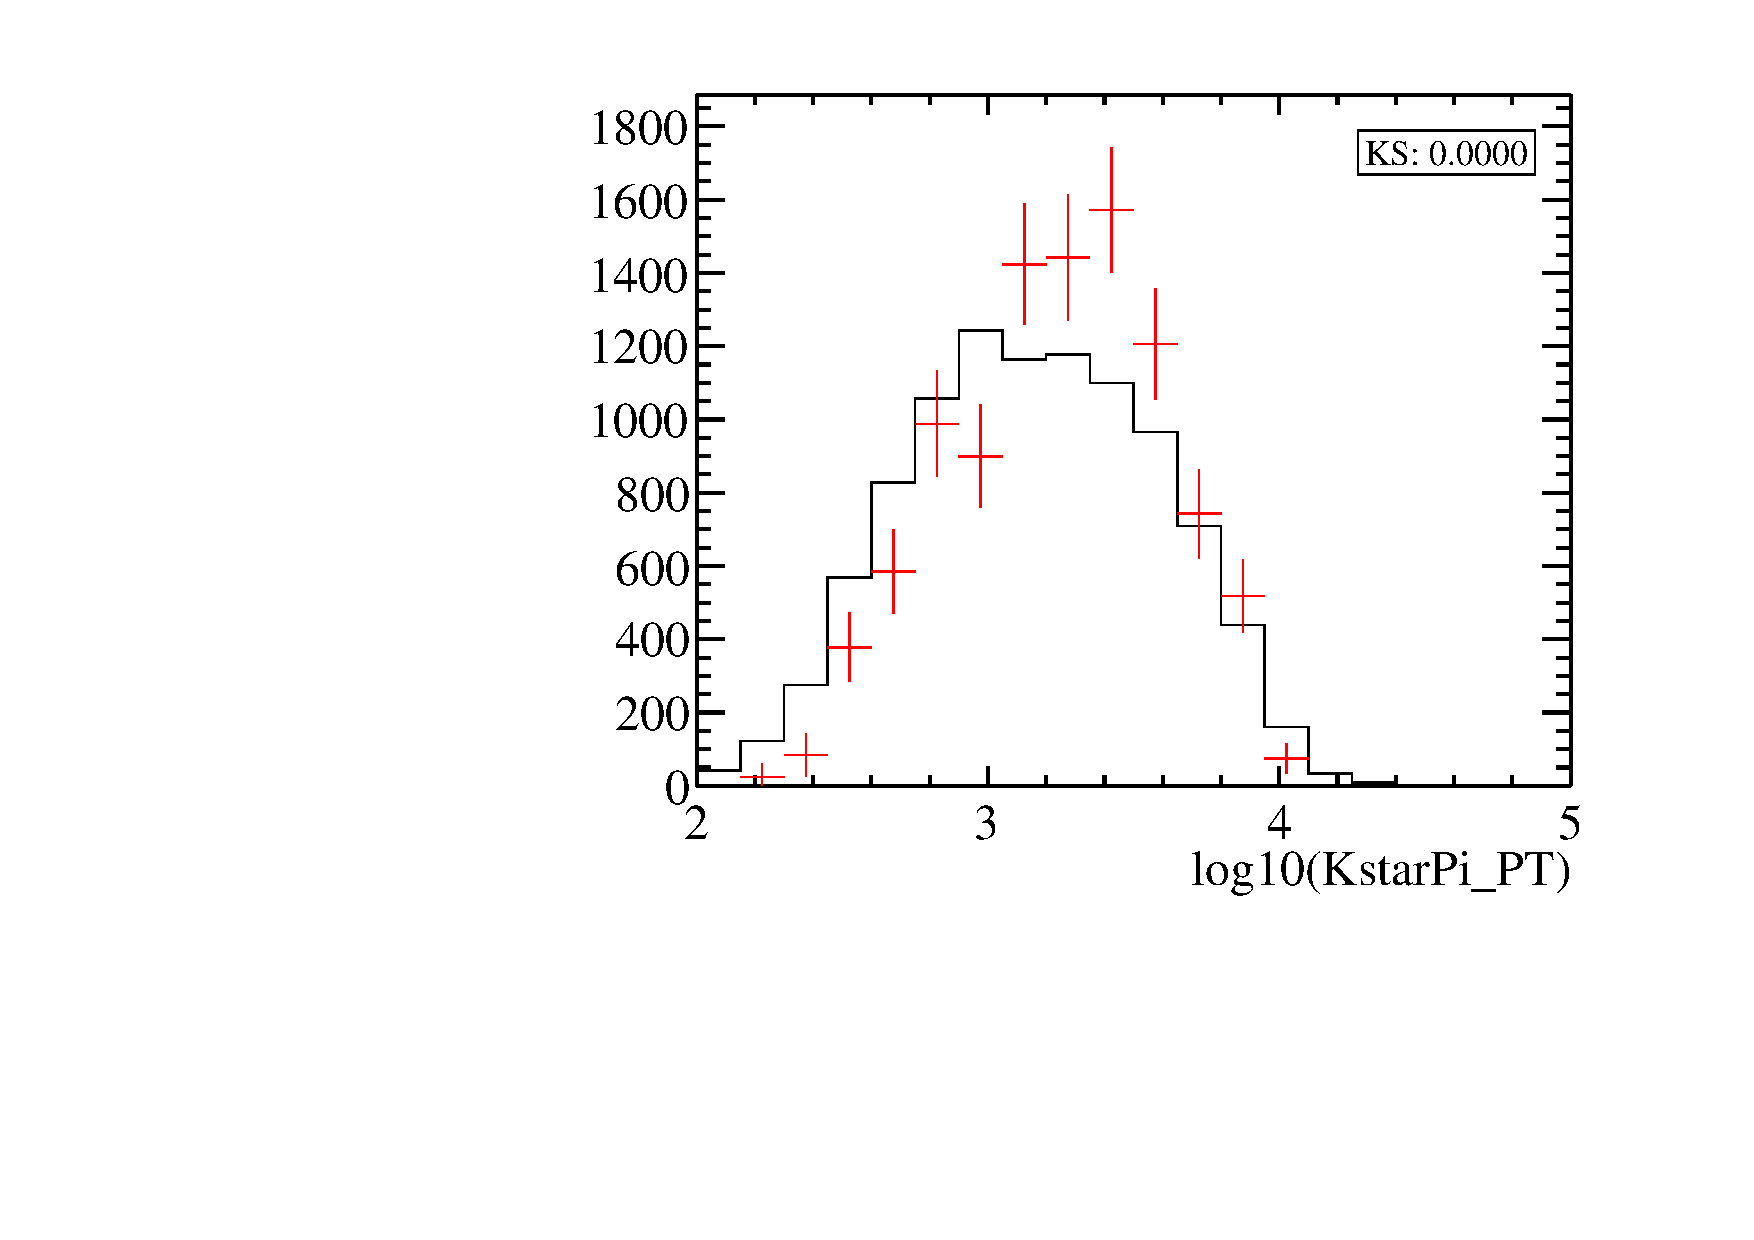
\includegraphics[width=0.3\textwidth]{ANA_resources/Plots/Monte_carlo/data_vs_MC/Kpipipi/log10(KstarPi_PT)_2016.pdf} \\
\end{tabular}
\caption{Comparison of 2016 data (red points) and Monte Carlo (black histogram) in the $K\pi\pi\pi$ mode for the variables used to train the $K\pi\pi\pi$ BDT. The result of the Kolmogorov Smirnov test on the two histograms is shown in the top-right corner of each plot}
\label{fig:data_vs_MC_Kpipipi_2016}
\end{figure}
